\documentclass[serif,xcolor=pdftex,dvipsnames,table,hyperref={bookmarks=false,breaklinks}]{beamer}

%%%%%%%%%%%%%%%%
% Change the macros below to configure the title slides
% for your course.
\newcommand{\coursename}{COMPSCI 590N}
\newcommand{\instructor}{Roy J. Adams}
\newcommand{\university}{University of Massachusetts Amherst}
\newcommand{\department}{College of Information and Computer Sciences}
%%%%%%%%%%%%%%%%

\newcommand\HUGE{\@setfontsize\Huge{50}{60}}

\newcommand{\settitlecard}[2]{
  \title[\coursename  Lecture #1] 
    {\coursename \\ Lecture #1: #2}
     \author[\instructor]{\instructor}
     \institute[\university]{
     \department\\
     \university
   }
\date{}
}

\newcommand{\maketitlepage}{
  \begin{frame}
  \titlepage
  %\center{
    %If you use the slides unmodified, retain the attribution below
  %  \tiny{Slides by Roy J. Adams (rjadams@cs.umass.edu). 
    %If you modify the slides, please retain the alternate attribution below
    %\tiny{Based on slides by Roy J. Adams (rjadams@cs.umass.edu). \\    
  %  }                                              
  %}  
  \end{frame}
}

\AtBeginSection[]
{
  \begin{frame}<beamer>{Outline}
    \tableofcontents[currentsection,subsectionstyle=hide]
  \end{frame}
}


\newcommand{\cut}[1]{}

\newcommand{\iconbox}[4]{
  \only<#1-#2>{
    \begin{columns}[T]
      \column{0.5in}
           \includegraphics[width=0.5in]{#3}
       \column{3.7in}
            #4
    \end{columns}
    \medskip
    \medskip
    \medskip
  }
}

\mode<presentation>{
  \usepackage{../beamertheme589theme}
  \setbeamercovered{invisible}
}

\mode<handout>{
  \usepackage{../beamertheme589theme}
  \setbeamercovered{transparent}
}


\usepackage[english]{babel}
\usepackage[latin1]{inputenc}
\usepackage{times}
\usepackage[T1]{fontenc}
\usepackage{amsmath}
\usepackage{amssymb}
\usepackage[noend]{algorithmic}
\usepackage{algorithm}
\usepackage{listings}
\usepackage{tcolorbox}
\usepackage{xmpmulti}

\renewcommand\mathfamilydefault{\rmdefault}

\newcommand{\setA}{\mathcal{A}}
\newcommand{\setB}{\mathcal{B}}
\newcommand{\setS}{\mathcal{S}}
\newcommand{\setV}{\mathcal{V}}
\DeclareMathOperator*{\union}{\bigcup}
\DeclareMathOperator*{\intersection}{\bigcap}
\DeclareMathOperator*{\Val}{Val}
\newcommand{\mbf}[1]{{\mathbf{#1}}}
\DeclareMathOperator*{\argmax}{arg\,max}
\DeclareMathOperator*{\argmin}{arg\,min}
\DeclareMathOperator*{\sign}{sign}
\newcommand{\deriv}[2]{\frac{\partial{#1}}{\partial{#2}}}

\lstdefinestyle{custompython}{
  belowcaptionskip=1\baselineskip,
  breaklines=true,
  frame=single,
  xleftmargin=\parindent,
  language=Python,
  showstringspaces=false,
  basicstyle=\footnotesize\ttfamily,
  keywordstyle=\bfseries\color{green!40!black},
  commentstyle=\itshape\color{purple!40!black},
  identifierstyle=\color{blue},
  stringstyle=\color{orange},
}
\lstset{style=custompython}

\makeatletter
\renewcommand*\env@matrix[1][*\c@MaxMatrixCols c]{%
  \hskip -\arraycolsep
  \let\@ifnextchar\new@ifnextchar
  \array{#1}}
\makeatother

\newcommand\norm[1]{\left\lVert#1\right\rVert}


\settitlecard{8}{Numerical Linear Algebra 2}

\begin{document}

\maketitlepage

% \section{Announcements}
% \subsection{Foo}
%
%
% \begin{frame}[t]{Announcements}
% 	\begin{itemize}
% 		\item Assignment 3 is due tonight at 11:55pm.
% 		\item Quiz 4 will go out tonight.
% 		\item Assignment 4 will go out in the next couple of days.
% 		\item Guest lecturer on Tuesday.
% 	\end{itemize}
% \end{frame}

\section{Numerical Linear Algebra 2}
\subsection{Foo}

\begin{frame}[t]{Matrix Inversion}
	% Review
	% Where it is used
	Review: An $n\times n$ square matrix $A$ is said to be \textbf{invertible} if there exists an $n \times n$ matrix $B$ such that:
	
	$$ AB = BA = I$$
	
	where $I$ is the identity matrix. If $B$ exists it is called the \textbf{inverse} and is denoted $A^{-1}$. Matrix inversion is the process of finding $A^{-1}$ for a given matrix $A$.
\end{frame}
	
\begin{frame}[t]{Matrix Inversion: Applications}
	\begin{itemize}[<+->]
		\item Matrix inverses appear in statistics frequently. Part of the reason for this is because of the appearance of a matrix inverse in the PDF of the multivariate normal distribution. 
		
		$$ \mathcal{N}(x;\mu,\Sigma) \propto \exp\left(-\frac{1}{2}(x-\mu)^T \Sigma^{-1}(x - \mu)\right) $$
		\item The analytical solution for least-squares linear regression involves a matrix inverse.
		\item Matrix inversion plays a fundamental role in many computer graphics routines.
		\item Matrix inversion is a subroutine for many more complex linear algebra computations.
	\end{itemize}
\end{frame}

\begin{frame}[t]{Gauss-Jordan Elimination}
	% Description
	\begin{itemize}[<+->]
		\item Many algorithms exist for inverting a matrix.
		\item We will analyze one of the fundamental algorithms called \textbf{Gauss-Jordan Elimination}.
		\item \textbf{Gaussian Elimination} is a method for solving equations of the form $Ax = b$ where $A$ is a matrix, $b$ is a vector, and we are solving for the vector $b$.
		\item Gaussian elimination can be thought of as a systematic application of simple substitution rules.
		\item Gauss-Jordan elimination is the application of this idea to the equation $AX = I$ where now $X$ is a matrix rather than a vector.
	\end{itemize}
\end{frame}

\begin{frame}[t]{Gauss-Jordan Elimination}
	% 2x2 example
	We'll start with a simple example: Let $A$ be the following $2 \times 2$ matrix.
	
	\pause
	$$A = \begin{bmatrix}[rr]
    	1 & 3 \\
		2 & 5
	\end{bmatrix}$$
	
	\pause
	Our goal is to find the inverse.
	\pause
	$$A^{-1} = \begin{bmatrix}[rr]
    	-5 & 3 \\
		2 & -1
	\end{bmatrix}$$
	
\end{frame}

\begin{frame}[t]{Gauss-Jordan Elimination}
	% 2x2 example
	We begin by writing $A$ in the following augmented form:
	
	\pause
	$$A = \begin{bmatrix}[rr|rr]
    	1 & 3 & 1 & 0\\
		2 & 5 & 0 & 1
	\end{bmatrix}$$
	
	\pause
	We then apply elementary row operations until the left side is equal to the identity matrix. Elementary row operations include:
	\pause
	\begin{itemize}[<+->]
		\item Scaling a row by a non-zero constant.
		\item Adding a scaled row to another row.
		\item Swapping two rows (we will not use this).
	\end{itemize}
	
	\pause
	If we are able to do this without getting a row of all zeros on the left, then the right side will be $A^{-1}$. If at any point we get a row with all zeros, then the matrix has no inverse.
	
\end{frame}

\begin{frame}[t]{Gauss-Jordan Elimination}
	% 2x2 example
	$$\begin{bmatrix}[rr|rr]
    	1 & 3 & 1 & 0\\
		2 & 5 & 0 & 1
	\end{bmatrix}$$
	
	\pause
	$$R_2 \leftarrow R_2 - 2R_1$$
	
	\pause
	$$\begin{bmatrix}[rr|rr]
    	1 & 3 & 1 & 0\\
		0 & -1 & -2 & 1
	\end{bmatrix}$$
	
\end{frame}

\begin{frame}[t]{Gauss-Jordan Elimination}
	% 2x2 example
	$$\begin{bmatrix}[rr|rr]
    	1 & 3 & 1 & 0\\
		0 & -1 & -2 & 1
	\end{bmatrix}$$
	
	\pause
	$$R_2 \leftarrow -R_2$$
	
	\pause
	$$\begin{bmatrix}[rr|rr]
    	1 & 3 & 1 & 0\\
		0 & 1 & 2 & -1
	\end{bmatrix}$$
	
\end{frame}

\begin{frame}[t]{Gauss-Jordan Elimination}
	% 2x2 example
	$$\begin{bmatrix}[rr|rr]
    	1 & 3 & 1 & 0\\
		0 & 1 & 2 & -1
	\end{bmatrix}$$
	
	\pause
	$$R_1 \leftarrow R_1 - 3R_2$$
	
	\pause
	$$\begin{bmatrix}[rr|rr]
    	1 & 0 & -5 & 3\\
		0 & 1 & 2 & -1
	\end{bmatrix}$$
	
	\pause
	\centering
	\Huge{Done!}
\end{frame}

% \begin{frame}[t]{Gauss-Jordan Elimination}
% 	% 2x2 example
% 	$$\begin{bmatrix}[rr|rr]
%     	1 & 0 & -5 & 3\\
% 		0 & 1 & 2 & -1
% 	\end{bmatrix}$$
%
% 	\pause
% 	\centering
% 	\Huge{Done!}
%
% \end{frame}

\begin{frame}[t]{Gauss-Jordan Elimination}
	% 2x2 example
	With such a small matrix it is hard to get a sense for what the steps are:
	\pause
	\begin{itemize}[<+->]
		\item For each row $i$ from top to bottom:
		\begin{itemize}[<+->]
			\item Scale the row so that the diagonal entry equals 1.
			\item Subtract a scaled version of row $i$ from each row below $i$ so that the $i$th column in each of these rows is $0$.
			\item This eliminates all entries below the diagonal and sets the diagonal to ones.
		\end{itemize}
		\item Repeat this process from the bottom up, this time eliminating entries above the diagonal.
	\end{itemize}
\end{frame}

\begin{frame}[t]{Gauss-Jordan Elimination}
	% 2x2 example
	$$A = \begin{bmatrix}[rrr]
    	2 & 3 & 0\\
		1 & -2 & -1\\
		2 & 0 & -1
	\end{bmatrix}$$
	
\end{frame}

\begin{frame}[t]{Gauss-Jordan Elimination}
	% 2x2 example
	$$\begin{bmatrix}[rrr|rrr]
    	2 & 3 & 0 & 1 & 0 & 0\\
		1 & -2 & -1 & 0 & 1 & 0\\
		2 & 0 & -1 & 0 & 0 & 1
	\end{bmatrix}$$
	
	\pause
	\begin{align*}
		R_1 &\leftarrow \frac{1}{2}R_1\\
	\end{align*}
	
	\pause
	$$\begin{bmatrix}[rrr|rrr]
    	1 & \frac{3}{2} & 0 & \frac{1}{2} & 0 & 0\\
		1 & -2 & -1 & 0 & 1 & 0\\
		2 & 0 & -1 & 0 & 0 & 1
	\end{bmatrix}$$
	
\end{frame}

\begin{frame}[t]{Gauss-Jordan Elimination}
	% 2x2 example
	$$\begin{bmatrix}[rrr|rrr]
    	1 & \frac{3}{2} & 0 & \frac{1}{2} & 0 & 0\\
		1 & -2 & -1 & 0 & 1 & 0\\
		2 & 0 & -1 & 0 & 0 & 1
	\end{bmatrix}$$
	
	\pause
	\begin{align*}
		R_2 &\leftarrow R_2 - R_1\\
		R_3 &\leftarrow R_3 - 2R_1\\
	\end{align*}
	
	\pause
	$$\begin{bmatrix}[rrr|rrr]
    	1 & \frac{3}{2} & 0 & \frac{1}{2} & 0 & 0\\
		0 & -\frac{7}{2} & -1 & -\frac{1}{2} & 1 & 0\\
		0 & -\frac{6}{2} & -1 & -1 & 0 & 1
	\end{bmatrix}$$
	
\end{frame}

\begin{frame}[t]{Gauss-Jordan Elimination}
	% 2x2 example
	$$\begin{bmatrix}[rrr|rrr]
    	1 & \frac{3}{2} & 0 & \frac{1}{2} & 0 & 0\\
		0 & -\frac{7}{2} & -1 & -\frac{1}{2} & 1 & 0\\
		0 & -\frac{6}{2} & -1 & -1 & 0 & 1
	\end{bmatrix}$$
	
	\pause
	\begin{align*}
		R_2 &\leftarrow -\frac{7}{2}R_2\\
	\end{align*}
	
	\pause
	$$\begin{bmatrix}[rrr|rrr]
    	1 & \frac{3}{2} & 0 & \frac{1}{2} & 0 & 0\\
		0 & 1 & \frac{2}{7} & \frac{1}{7} & -\frac{2}{7} & 0\\
		0 & -\frac{6}{2} & -1 & -1 & 0 & 1
	\end{bmatrix}$$
	
\end{frame}

\begin{frame}[t]{Gauss-Jordan Elimination}
	% 2x2 example
	$$\begin{bmatrix}[rrr|rrr]
    	1 & \frac{3}{2} & 0 & \frac{1}{2} & 0 & 0\\
		0 & 1 & \frac{2}{7} & \frac{1}{7} & -\frac{2}{7} & 0\\
		0 & -\frac{6}{2} & -1 & -1 & 0 & 1
	\end{bmatrix}$$
	
	\pause
	\begin{align*}
		R_3 &\leftarrow R_3 + \frac{6}{2}R_2\\
		R_3 &\leftarrow -7R_3
	\end{align*}
	
	\pause
	$$\begin{bmatrix}[rrr|rrr]
    	1 & \frac{3}{2} & 0 & \frac{1}{2} & 0 & 0\\
		0 & 1 & \frac{2}{7} & \frac{1}{7} & -\frac{2}{7} & 0\\
		0 & 0 & 1 & -4 & -6 & -7
	\end{bmatrix}$$
	
\end{frame}

\begin{frame}[t]{Gauss-Jordan Elimination}
	% 2x2 example
	$$\begin{bmatrix}[rrr|rrr]
    	1 & \frac{3}{2} & 0 & \frac{1}{2} & 0 & 0\\
		0 & 1 & \frac{2}{7} & \frac{1}{7} & -\frac{2}{7} & 0\\
		0 & 0 & 1 & -4 & -6 & -7
	\end{bmatrix}$$
	
	\pause
	\begin{align*}
		R_2 &\leftarrow R_2 - \frac{2}{7}R_3\\
		R_1 &\leftarrow R_1 + 0R_3\\
	\end{align*}
	
	\pause
	$$\begin{bmatrix}[rrr|rrr]
    	1 & \frac{3}{2} & 0 & \frac{1}{2} & 0 & 0\\
		0 & 1 & 0 & -1 & -2 & 2\\
		0 & 0 & 1 & -4 & -6 & -7
	\end{bmatrix}$$
	
\end{frame}


\begin{frame}[t]{Gauss-Jordan Elimination}
	% 2x2 example
	$$\begin{bmatrix}[rrr|rrr]
    	1 & \frac{3}{2} & 0 & \frac{1}{2} & 0 & 0\\
		0 & 1 & 0 & -1 & -2 & 2\\
		0 & 0 & 1 & -4 & -6 & -7
	\end{bmatrix}$$
	
	\pause
	\begin{align*}
		R_1 &\leftarrow R_1 - \frac{3}{2}R_2\\
	\end{align*}
	
	\pause
	$$\begin{bmatrix}[rrr|rrr]
    	1 & 0 & 0 & 2 & 3 & -3\\
		0 & 1 & 0 & -1 & -2 & 2\\
		0 & 0 & 1 & -4 & -6 & -7
	\end{bmatrix}$$
	
	\pause
	\centering
	\Huge{Done!}
	
\end{frame}

\begin{frame}[t]{Gauss-Jordan Complexity}
	% Complexity
	% n multiplications
	% n multiplications
	% (n - i)*n additions
	\pause
	\begin{itemize}[<+->]
		\item When you scale a row so that its diagonal is one, how many multiplications do we perform? How many times do we do this?
		\begin{itemize}[<+->]
			\item $n$ multiplications. One per item in the row.
			\item $n$ times. Once per row.
		\end{itemize}
		\item When performing a row reduction (adding one scaled row to another), how many multiplications and additions do we perform? How many many rows to we add row $i$ to?
		\begin{itemize}
			\item $n$ multiplications. (technically $n-i$)
			\item $n$ additions. (technically $n-i$)
			\item We add row $i$ to all rows below row $i$, so $n-i$ times.
		\end{itemize}
	\end{itemize}
\end{frame}

\begin{frame}[t]{Gauss-Jordan Complexity}
	\begin{align*}
		\onslide<1->{\text{No. Operations } &= 2\sum_{i=1}^{n}\left(n + 2n(n-i)\right)\\}
		\onslide<2->{&= 2\sum_{i=1}^{n}\left(n + 2n^2 - 2ni\right)\\}
		\onslide<3->{&= 2\left[\sum_{i=1}^{n}n + 2\sum_{i=1}^{n}n^2 - 2\sum_{i=1}^{n}ni\right]\\}
		\onslide<4->{&= 2\left[n^2 + 2n^3 - 2n\frac{n(n+1)}{2}\right]\\}
		\onslide<5->{&= 2\left[n^2 + 2n^3 - n^3 + n^2\right]\\}
		\onslide<6->{&= 4n^2 + 2n^3} \onslide<7>{= \mathcal{O}(n^3)}
	\end{align*}
	
\end{frame}

\begin{frame}[t]{Advanced Matrix Inverse Algorithms}
	% Description
	As with matrix multiplication, more sophisticated algorithms exist the have complexity between $n^2$ and $n^3$.
\end{frame}

\begin{frame}[t]{Estimating the complexity of NumPy Matrix Inverse}
	% Fit a line
	The algorithm used by NumPy is not well documented. How could we estimate its complexity? \pause(Hint: We know the complexity is approximately a monomial (e.g. $\mathcal{O}(n^3)$)).
	
	\pause
	\begin{align*}
		\text{Run time } &\approx Cn^b\\
		\log(\text{Run time}) &\approx \log(C) + b\log(n)
	\end{align*}
	
	\pause
	Solution: 
	\begin{enumerate}
		\item Run a bunch of tests for different $n$ and record the run times.
		\item Fit a line to the $\log$ run times. The slope will be the degree of the polynomial and the intercept will be the logged constant.
	\end{enumerate}
	 
\end{frame}


\begin{frame}[t]{Estimating the complexity of NumPy Matrix Inverse}
	% Fit a line
	\centering
	\Huge{Demo}
\end{frame}

\begin{frame}[t]{Eigenreview}
	% Description
	% Eigen Review
	Let $A$ be a square $n\times n$ matrix, then the $\mathbf{v}$ is an \textbf{eigenvector} of $A$ if
	
	$$A\mathbf{v} = \lambda\mathbf{v}$$
	
	for some constant $\lambda$ known as an \textbf{eigenvalue}. \textbf{Eigen decomposition} is the process of finding the eigenvalue/eigenvector pairs of a matrix.
\end{frame}

\begin{frame}[t]{Eigen Decomposition: Applications}
	% Description
	% Eigen Review
	\begin{itemize}[<+->]
		\item Eigen decompositions are used in many practical applications:
		\begin{itemize}[<+->]
			\item Google's PageRank computes the largest eigenvalue/vector pair.
			\item Principal Components Analysis (PCA) is used in many data analysis settings to reduce the dimensionality of a dataset and reduce collinearity.
			\item Spectral clustering is used in machine learning and computer vision for clustering data points and parts of images. Spectral clustering requires calculating the Eigen decomposition of a similarity matrix.
		\end{itemize}
	\end{itemize}
\end{frame}

\begin{frame}[t]{Eigen Decomposition: Eigenfaces}
	% Description
	% Eigen Review
	\begin{itemize}[<+->]
		\item One of the seminal early pieces of work in computer vision worked by compressing images into eigenvectors.
		\item The basic idea was to calculate the number of images by number of images image covariance matrix and computing the eigenvectors of this matrix.
		\item The result is one eigenvector for each image.
		\item The most well known application was facial recognition where each image was of a face, hence eigenfaces.
	\end{itemize}
	
	\pause
	\centering
	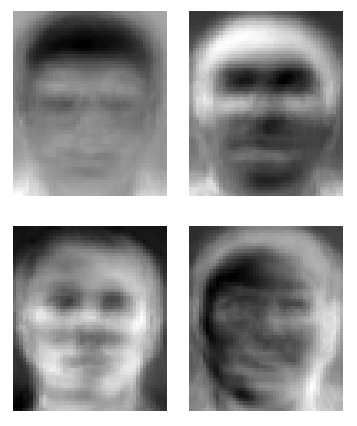
\includegraphics[height=1in]{{../Figures/Eigenfaces}.png}
\end{frame}

\begin{frame}[t]{Eigen Decomposition: The Power Method}
	% Description
	The Power method is a method for calculating the eigenvalue corresponding to the greatest eigenvalue. Many other methods for calculating the full set of eigenvalues are generalizations of this method.
	
	\pause
	\begin{block}{The Power Method}
		\begin{enumerate}[<+->]
			\item Given an $n\times n$ matrix $A$, choose a random initial vector $b_0$.
			\item Then, under some mild assumptions, the following sequence will converge to the dominant eigenvector:
			
			$$\frac{Ab_0}{\norm{Ab_0}},\frac{A^2b_0}{\norm{A^2b_0}},\frac{A^3b_0}{\norm{A^3b_0}},...$$
		\end{enumerate}
	\end{block}
	
\end{frame}

\begin{frame}[t]{Eigen Decomposition: Complexity}
	% Description
	If we were to calculate matrix matrix powers $A^k$ directly using matrix multiplication, what is the complexity of calculating $A^k$?
	
	\pause
	\begin{itemize}
		\item Answer: We would need to perform $k$ matrix multiplications, thus using Strassen's this would take $\approx\mathcal{O}(kn^{2.807})$.
	\end{itemize}
	
	\pause
	Fortunately, there is a better way. We can use the following interative algorithm:
	
	$$b_{k} = \frac{A^kb_0}{\norm{A^kb_0}} = \frac{A(A^{k-1}b_0)}{\norm{A(A^{k-1}b_0)}} = \frac{Ab_{k-1}}{\norm{Ab_{k-1}}}$$
	
	\pause
	What is the complexity of computing $Ab_{k-1}$?
	
	\pause
	\begin{itemize}
		\item The power method has complexity $\mathcal{O}(n^2)$ \textbf{per iteration}.
	\end{itemize}
\end{frame}

\begin{frame}[t]{Inversion and Decomposition in Action: Linear Regression}
	% Linear Regression Derivation
	Let $X \in \mathbb{R}^{n\times m}$ be a $n \times m$ matrix of data cases (i.e. design matrix) and let $y \in \mathbb{R}^n$ be a length $n$ vector of real values. Then in ordinary least squares linear regression, we have the following model:

	$$y = \beta X + \epsilon$$

	where $\epsilon$ is a normally distributed vector of noise. \pause Then using Maximum Likelihood Estimation, we estimate $\hat{\beta}$ as

	$$\hat{\beta} = \argmin_\beta (\beta X - y)^T(\beta X - y)$$
	
\end{frame}

\begin{frame}[t]{Inversion and Decomposition in Action: Linear Regression}
	% Linear Regression Derivation
	The solution to this minimization problem can be found by taking the gradient with respect to $\beta$, setting it to zero, and solving. The results is:
	
	$$\hat{\beta} = (X^T X)^{-1}X^Ty$$
	
	\pause
	\begin{itemize}[<+->]
		\item We can solve this using just matrix inversion and matrix multiplication.
		\item The advanced linear algebraist may have noticed that $(X^T X)^{-1} X^T$ is called the \textbf{Moore-Penrose pseudoinverse}.
		\item There are specialized algorithms for computing the Moore-Penrose pseudoinverse.
		\item Part of Assignment 4 will be implementing and comparing linear regression using straight inversion vs. pseudoinversion.
	\end{itemize}

\end{frame}

% \begin{frame}[t]{Inversion and Decomposition in Action: Linear Regression}
% 	% Demo
% 	\centering
% 	\Huge{Demo}
% \end{frame}

\begin{frame}[t]{Linear Algebra in NumPy}
	NumPy has a sub-module called \textbf{numpy.linalg} which implements the following groups of methods:
	\pause
	\begin{itemize}[<+->]
		\item Products: inner, outer, matrix, etc.
		\item Decompositions: Cholesky, QR, SVD, Eigen
		\item Special numbers: rank, norm, determinant, etc.
		\item Solvers: Inversion, solve $Ax = b$, least squares, pseudoinversion, etc.
		\item Plus a few more...
	\end{itemize}
\end{frame}

\begin{frame}[t]{Numerical Linear Algebra: Major Takeaways}
	\begin{itemize}[<+->]
		\item If you continue to do numerical computing, you will likely find yourself using some of these linear algebra computations.
		\item Keep the approximate complexities for the major methods in mind so that you know what is feasible in your programs.
		\begin{itemize}[<+->]
			\item For example: Directly solving linear regression with 1,000 instances is feasible, but 1,000,000 might not be. In this case you should consider a different method.
		\end{itemize}
		\item As a rule of thumb, assume $\mathcal{O}(n^3)$ runtime.
		\item Approximations for many of these computations exist that are good enough in many cases.
	\end{itemize}
\end{frame}

% \begin{frame}[t]{Eigen Decomposition: QR Algorithm}
% 	% Description
% \end{frame}
%
% \begin{frame}[t]{Eigen Decomposition: QR Algorithm}
% 	% Description
% \end{frame}

% \section{Sparse Matrices}
% \subsection{Foo}

\end{document}
